\newpage
\section{Daten Generierung} \label{ch:generation}

Für die Analyse von Datenintervallen werden Testdaten benötigt, welche auf die verschiedenen Muster untersucht werden können. Aus diesem Zusammenhang wurde im Rahmen dieser Arbeit eine Anwendung programmiert, welche je nach Parameterangaben verschiedene Testdateien generieren kann. Dabei gilt, dass 0 der Normalzustand ist und 1 einen Problemzustand darstellt.

\needspace{6\baselineskip}
Bei dieser Anwendung handelt es sich um eine Konsolenapplikation, welche in C\texttt{\#} mit dem .NET Core Framework geschrieben wurde. Durch die Verwendung von .NET Core wird sichergestellt, dass das Programm neben Windows auch auf Mac und Linux mit vollem Umfang lauffähig ist. 

\needspace{6\baselineskip}
Der Benutzer gibt der Anwendung seine Einstellungen entweder über Kommandozeilenparameter (siehe Abbildung \autoref{fig:commando}) mit oder über die Konsolenanwendung, welche nach den nicht angegebenen Parametern frägt. Das Ergebnis wird in einer CSV-Datei in unserem Format (siehe \autoref{ch:format}) abgespeichert. Der Ablaufprozess wird in \autoref{fig:genUml} verdeutlicht.

\vspace{20pt}
\needspace{6\baselineskip}
\begin{figure}[tbph]
	\centering 
	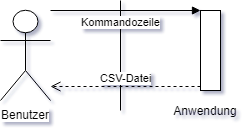
\includegraphics[width=0.6\textwidth,keepaspectratio] {dataPreparation/images/generationUml.png} 
	\caption{\label {fig:genUml} Use-Case-Diagramm der Generationsanwendung} 
\end{figure}


\vspace{20pt}
\needspace{6\baselineskip}
\begin{figure}[tbph]
	\centering 
	
\includegraphics[width=0.9\textwidth,keepaspectratio] {dataPreparation/images/commando.png} 
	\caption{\label {fig:commando} Aufruf des Programmes mit Kommandozeilenparameter} 
\end{figure}

\newpage
\needspace{8\baselineskip}
Als Parameter für die Anwendung gibt es verschieden Optionen, welche das Programm zum Start benötigt. Dabei handelt es sich um folgende:

\vspace{10pt}
\begin{description} 
	\item[IntervalsMaximum] \hfill \\ Integer, gibt die Anzahl der Intervalle an, welche generiert werden. Der Standartwert liegt hier bei 10000.
	\item[IsHighfrequent] \hfill \\ Nullable Boolean, kann die Generation beeinflussen, ob eher hochfrequente oder nieder frequente Sequenzen herauskommen. Kann auf null gesetzt werden um die Generation dem Zufall zu überlassen.
	\item[UsePattern] \hfill \\ Boolean, gibt an, ob bei der Generation willkürlich generiert werden soll oder bestimmte Muster (\enquote{Patterns}) genutzt werden sollen.
	\item[UseComplexRandom] \hfill \\ Boolean, der die Nutzung einer komplexeren Zufallsmethode angibt. Dies führt jedoch zu längeren Berechnungszeiten, weshalb er standardmäßig aus ist.
	\item[UseShortSaveForm] \hfill \\ Boolean, gibt an, ob die Kurzform des Speichersystemes genutzt werden soll (wie in \autoref{ch:format} beschrieben)
\end{description} 

\subsection{Algorithmus zur Datengenerierung}

Für die eigentliche Generierung der Daten wird ein Algorithmus verwendet, welcher im Zweck dieser Arbeit entstanden ist. Zuerst werden die mitgegebenen Parameter ausgelesen und analysiert. Dadurch können Optionen gesetzt werden, wie die maximale Länge eines Pattern (dt. Muster), die Häufigkeit von Patterns in der Sequenz und die möglichen Patterns.

\needspace{6\baselineskip}
Ein Pattern ist die Abfolge bestimmter 0 und 1 Kombinationen, welche wiederholt auftreten. Zwischen diesen Patterns befinden sich eine große Ansammlung von 0, da angenommen wird, dass die theoretische Maschine in diesen Zeiträumen ordnungsgemäß funktioniert. Durch den Parameter \enquote{IsHighfrequent} werden die Parameter auf die Frequenz beeinflusst, wodurch die Chance höher oder tiefer ist, dass entsprechende Frequenzen vorliegen.

\needspace{6\baselineskip}
Diese Patterns wurden im Zuge der Studienarbeit erstellt, damit eine Ähnlichkeit zwischen den generierten Intervallen und den maschinellen Daten besteht. Ein Pattern stellt hierbei eine gewisse Art von Problem dar, welche bei einer realen Maschine hätte auftreten können. Diese helfen zudem, dass in den computergenerierten Daten eine Form der Korrelation festgestellt werden kann, was bei zufällig generierten Daten nicht unbedingt gegeben wäre. 

\needspace{6\baselineskip}
Grundlegend geben die Patterns die Intervallmöglichkeiten an, welche bereits im vorangegangenen Kapitel erklärt wurden. Im Folgenden ist eine Liste aller möglichen Patterns:

\needspace{6\baselineskip}
\vspace{10pt}
\begin{description} 
	\item[Peak] \hfill \\ Einzelner Ausschlag von 1-5 Fehlerzuständen. Hierbei kann es sich um einen Messfehler oder ein kleines Problem handeln, welches sich sofort selbst behebt.
	\item[Block] \hfill \\ Langer Auschlag von 20-500 Fehlerzuständen. Symbolisiert ein größeres Problem, bei dem die Maschine stehen geblieben ist und nicht mehr funktioniert.
	\item[Shiver] \hfill \\ Schneller Wechsel von Funktionsfähigkeit und Fehlerzustand in 1-3er Abständen. Zeigt ein Problem, bei dem die Maschine mit Behinderung läuft.
	\item[Long Shiver] \hfill \\ Langsamer Wechsel von Funktionsfähigkeit und Fehlerzustand in 5-20er Abständen. Ähnlich dem normalen Shiver, aber mit mehr Abstand um die Variation zu erhöhen.
	\item[Random] \hfill \\ Zufallsgenerierte Ansammlung von 0 und 1. Stellt eine nicht sofort erklärbare Situation dar, welche mit geringer Wahrscheinlichkeit jederzeit auftreten kann.
\end{description}


\vspace{10pt}
\needspace{6\baselineskip}
Der grundsätzliche Algorithmus funktioniert in drei Einzelabschnitten. Zuerst wird die Anzahl der Patterns ermittelt, welche für die maximale Intervallänge angemessen sind. Die genaue Zahl ist zufällig, wird allerdings von der Option \enquote{IsHighfrequent} erhöht, falls diese gesetzt wurde. Durch die zufällige Anzahl an Patterns ergibt sich eine größere Vielfalt an unterschiedlichen Intervallen.

\needspace{6\baselineskip}
Sobald die Anzahl der Patterns klar ist, wird deren Länge und Abstand geklärt. Die Länge gibt die Anzahl an Werten an, die ein Intervall beinhaltet, während der Abstand die Anzahl von 0 zwischen zwei Patterns angibt. Diese Anzahlen werden ebenfalls zufällig generiert um Varianz zu schaffen.

\needspace{6\baselineskip}
Der letzte Schritt ist das Zuordnen der verschiedenen Patterns auf die entstandenen Patternplätze. Die Patterns werden zufällig ausgelost, allerdings mit unterschiedlicher Wahrscheinlichkeit. Dabei wird vor allem auf die Option \enquote{IsHighfrequent} Rücksicht genommen, wodurch viele Shiver und wenige Blöcke oder Peaks ausgewählt werden. 

\needspace{6\baselineskip}
Im Anschluss werden die Patterns mit entsprechender Länge und Abstand eingefüllt und das Intervall wird vollständig gebildet. Falls \enquote{UseShortSaveForm} gesetzt wurde, wird das Intervall auf die kurze Schreibweise aus \autoref{ch:format} umgewandelt. Das Ergebnis wird in einer CSV-Datei gespeichert.